\documentclass[12pt, a4paper]{article}
\usepackage[utf8]{inputenc}
\usepackage{amsmath}
\usepackage{amsfonts}
\usepackage{amssymb}
\usepackage{graphicx}
\usepackage{caption}
\usepackage{subcaption}
\usepackage{sidecap}
\author{MORAES, FELIPE}
\title{Fundamentals of STDP based recurrent assembly networks}

\newtheorem{theorem}{Theorem}[section]
\newtheorem{lemma}[theorem]{Lemma}
\newtheorem{proposition}[theorem]{Proposition}
\newtheorem{corollary}[theorem]{Corollary}

\newenvironment{proof}[1][Proof]{\begin{trivlist}
\item[\hskip \labelsep {\bfseries #1}]}{\end{trivlist}}
\newenvironment{definition}[1][Definition]{\begin{trivlist}
\item[\hskip \labelsep {\bfseries #1}]}{\end{trivlist}}
\newenvironment{example}[1][Example]{\begin{trivlist}
\item[\hskip \labelsep {\bfseries #1}]}{\end{trivlist}}
\newenvironment{remark}[1][Remark]{\begin{trivlist}
\item[\hskip \labelsep {\bfseries #1}]}{\end{trivlist}}

\newcommand{\qed}{\nobreak \ifvmode \relax \else
      \ifdim\lastskip<1.5em \hskip-\lastskip
      \hskip1.5em plus0em minus0.5em \fi \nobreak
      \vrule height0.75em width0.5em depth0.25em\fi}

\renewcommand{\figurename}{Figura}

\begin{document}

\begin{center}
{\huge TRABALHO PRÁTICO 4: Editor de Ligação}

\textit{Felipe Moraes Gomes - felipemoraes@dcc.ufmg.br}
\end{center}

\section{Introdução e Definição do Trabalho}
Este trabalho descreve a implementação e operação de editor de ligação para uma linguagem assembly hipotética, baseada no conjunto de instruções do RISC. O editor recebe como entrada múltiplos arquivos, em um formato intermediário, contendo somente o que ele precisa para efetuar a ligação.


O restante deste documento está organizado da seguinte forma: A 2\textsuperscript{a} seção trata da implementação do montador e de sua organização no código; A 3\textsuperscript{a} seção resume o formato de execução, entrada e saída do programa; A 4\textsuperscript{a} seção contém os testes realizados; A 5\textsuperscript{a} seção conclui o trabalho. Após isso, é colocado um apêndice contendo uma listagem dos arquivos do projeto. 
	
\section{Implementação e Organização}

O editor funciona em 3 etapas. Primeiro, ele abre cada um dos arquivos objetos gerados pelo montador, e os carrega para a memória, a começar pelo main. Ao fazer isso, ele aloca o espaço que cada arquivo ocupará no executável gerado, gerando os offsets. Em seguida, a linkagem é feita, onde as referências irresolvidas são buscadas nos outros arquivos. Não havendo êxito na busca, o editor emite um erro. Finalmente, os arquivos fontes são realocados para o arquivo final, já com as dependêncidas resolvidas, e o executável é gerado.

\subsection{Dados e Variáveis}


\begin{itemize}
	\item \emph{Object}: Estrutura contendo o início e o fim do objeto; a tabela de referências conhecidas; a tabela de todas as referências; o tamanho do programa e o programa antes da alocação e linkagem. 


\subsection{Métodos e Funções}
\begin{itemize}
	\item \emph{void leituraObjetos(nome do arquivo de entrada, lista de estruturas objeto)}: Lê os dados dos módulos e monta cada estrutura objeto.
	\item \emph{void alocacao(lista de estruturas objeto, inteiro com o número de objetos)}: Aloca o espaço que cada arquivo ocupará no executável gerado, gerando os offsets.
	
	\item \emph{void realocacao(lista de estruturas objeto, inteiro com o número de objetos)}: As referências irresolvidas são buscadas nos outros arquivos.
	
\end{itemize}

\subsection{Fluxo de Execução}

O programa inicialmente lê os parâmetros passados a ele, verificando seu formato. Caso correto, ele cria um vetor da estrutura objeto associado a cada arquivo, e seta os offsets correspondetens. Após isso, as referências são resolvidas, e as instruções de cada objeto são inseridos em série no arquivo de saída (a começar pelo main, segundo então a ordem de entrada). Não havendo falhas neste processo, o main retorna 0.

\section{Controle \& IO}

\subsection{Execução e Compilação do Expansor}

O programa pode ser compilado através do g++, pelo utilitário \emph{make}, usando o makefile providenciado. Uma vez compilado, chamadas devem seguir o formato:

\begin{center}
\emph{./ligador n*[FonteN.mmk] [-m main.mmk] [-o Executável.mk]}
\end{center}

Onde se especifica uma quantidade variável de arquivos fonte FonteN.mmk, um único arquivo principal main.amk, prefixado por -m, e um arquivo de saída Executável.mk, prefixado por -o. Os termos podem aparecer em qualquer ordem.

\subsection{Formato dos Arquivos de Entrada e Saída}

Cada linha dos programas de entrada do ligador deve seguir o formato:

\begin{itemize}
\item Número de referências conhecidas daquele módulo

\item N referências conhecidas e seus ILCs

\item Número de referências totais daquele módulo

\item M número de referências totais daquele módulo e onde foram referênciadas naquele módulo.

\item X inteiros que representam o programa total, onde o inteiro 32767 representa uma referência desconhecida naquele módulo. 
\end{itemize}

Onde \emph{label} e \emph{comentário} são opcionais, porém devendo ser devidamente delimitados (o sufixo ``:'' para o label e o prefixo ``;'' para o comentário). O tipo e quantidade dos operandos é dependente da instrução.

\section{Testes}

\begin{figure}
\centering
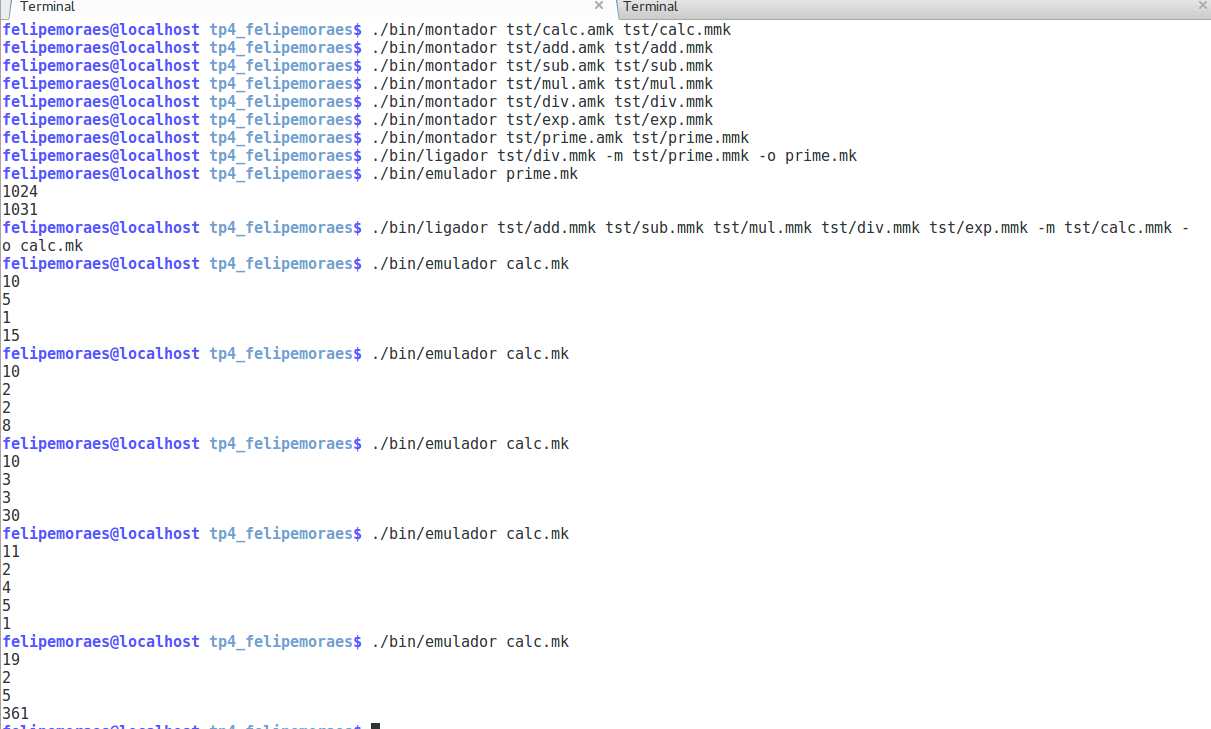
\includegraphics[width=1.5\textwidth]{screenshot.png}
\caption{Compilação e execução dos testes}
\label{FigureExecution}
\end{figure}

Vários programas foram testados, de forma a obter cobertura total do código. Os testes podem ser executados na MV tornando \emph{PC = EndInicial = 0} e \emph{SP = 1000}. Os testes fizeram forte uso do expansor de macros, que promove grandes alterações sintáticas, visando aproximar uma linguagem mais alta.

\begin{itemize}
	\item \emph{Calculadora (calc.amk):} Implementa uma calculadora simples, que recebe 3 parâmetros: operando A, operando B e o número que representa a operação. Faz-se (1) $A+B$, (2) $A-B$, (3) $A*B$, (4) $A/B$ e $A\%B$, (5) $A^B$.
	\item \emph{Primo (primo.amk):} Lê um valor do teclado e imprime o primeiro número primo maior que ele. Possui dependências com o módulo div.	
\end{itemize}

\section{Conclusão}

O ligador é eficaz em lidar com programas escritos neste conjunto de instruções, permitindo recompilação parcial e programas multi-modulares.

A execução do trabalho transcorreu sem maiores dificuldades, e os resultados obtidos correspondem ao esperado.

\appendix
\section{Apêndice}
\subsection{Listagem de Arquivos}
\begin{itemize}
	\item Código Fonte:
\begin{itemize}
\item \emph{src/main.c:} Interpreta os parâmetros de entrada e controla o fluxo do programa.
\item \emph{src/lista.c, src/lista.h:} Implementa TAD lista encadeada.
\item \emph{src/linker.c, src/linker.h:} Implementa o ligador.

\end{itemize}
	\item Testes:
	\begin{itemize}
		\item \emph{tst/calc.amk}
		\item \emph{tst/add.amk}
		\item \emph{tst/sub.amk}
		\item \emph{tst/mul.amk}
		\item \emph{tst/div.amk}
		\item \emph{tst/exp.amk}
		\item \emph{tst/prime.amk}
	\end{itemize}
	
\end{itemize}

\end{document}